\section{Linear Regression Model}

\subsection{One hot encoding}

Linear regression can only operate on numerical values. This caused an issue with the \textbf{Sex} column as it is not numeric. I had to use a technique called "one hot encoding" to transform the Sex column into a usable feature. Interestingly, one hot encoding does not merely transform the sex column into 1 for infant, 2 for male, 3 for female. Instead it creates three new features. These new features are F for female, I for infant and M for male. The feature can have a value of either 1 or 0, 1 meaning "is a" and 0 meaning "not a". For example if F has a value of 1 then we can say it is a female. Alternatively if F has a value of 0 then we can say it is not a female. The results can be seen in figure \ref{fig:abalone-one-hot-encoding}
\begin{figure}[H]
  \centering
  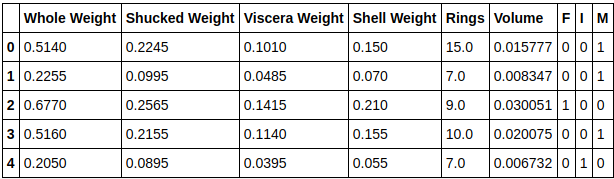
\includegraphics[scale=0.5,width=100mm]{./images/abalone-one-hot-encoding.png}
  \caption{Table showing the results of one hot encoding}
  \label{fig:abalone-one-hot-encoding}
\end{figure}

\subsection{Linear Regression}

\begin{figure}[H]
  \centering
  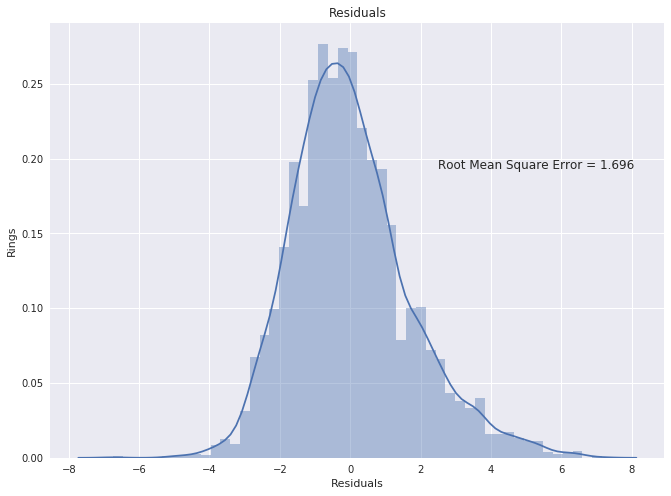
\includegraphics[scale=0.5,width=100mm]{./images/abalone-linear-regression-hist.png}
  \caption{Table showing the results of one hot encoding}
  \label{fig:abalone-one-hot-encoding}
\end{figure}